% Created 2024-04-08 Mon 21:18
% Intended LaTeX compiler: pdflatex
\documentclass[a4paper, 11pt]{article}
\usepackage[utf8]{inputenc}
\usepackage[T1]{fontenc}
\usepackage{graphicx}
\usepackage{longtable}
\usepackage{wrapfig}
\usepackage{rotating}
\usepackage[normalem]{ulem}
\usepackage{amsmath}
\usepackage{amssymb}
\usepackage{capt-of}
\usepackage{hyperref}
\usepackage{lmodern} % Ensures we have the right font
\usepackage[T1]{fontenc}
\usepackage{inputenc}
\usepackage{graphicx, float}
\usepackage{amsmath, amsfonts, amsthm, amssymb, lipsum}
\usepackage[table, xcdraw]{xcolor}
\usepackage[colorlinks]{hyperref}
\hypersetup{colorlinks, linkcolor=blue, urlcolor=blue}
\setlength{\parindent}{0pt}
\setlength{\parskip}{1em}
\usepackage[stretch=10]{microtype}
\usepackage{hyphenat}
\usepackage{ragged2e}
\usepackage{subfig} % Subfigures (not needed in Org I think)
\usepackage{hyperref} % Links
\usepackage{listings} % Code highlighting
\usepackage[margin=1in, footskip=0.25in]{geometry}
\renewcommand{\baselinestretch}{1.15}
\pagenumbering{gobble}
\usepackage[explicit]{titlesec}
\usepackage{enumitem}
\setlist[itemize]{topsep=0pt}
\newtheorem{theorem}{Theorem}[section]
\newtheorem{corollary}{Corollary}[theorem]
\newtheorem{lemma}[theorem]{Lemma}
\newtheorem{definition}{Definition}[theorem]
\setlength{\abovedisplayskip}{-15pt}
\setlength{\belowdisplayskip}{0pt}
\setlength{\abovedisplayshortskip}{0pt}
\setlength{\belowdisplayshortskip}{0pt}
\author{Bryan Lim Jing Xiang (A0233605M)}
\date{}
\title{Task B2}
\hypersetup{
 pdfauthor={Bryan Lim Jing Xiang (A0233605M)},
 pdftitle={Task B2},
 pdfkeywords={},
 pdfsubject={},
 pdfcreator={Emacs 29.3 (Org mode 9.7)}, 
 pdflang={English}}
\begin{document}

\maketitle
\section{Dataset}
\label{sec:orgbc4f2c7}
\subsection{Overview}
\label{sec:orgc89d7f7}
This dataset is produced by processing and combining the dataset of monthly COE bids and monthly COE revalidation for cars in Singapore in recent years. The data fields of interest here are:

\begin{center}
\begin{tabular}{lll}
Field & Description & Data Type\\[0pt]
\hline
Month & Month and Year of the data point & String\\[0pt]
bids\textsubscript{received} & Number of COE bids that month & Integer\\[0pt]
quota & COE quota that month & Integer\\[0pt]
bids\textsubscript{success} & Number of successful bids that month & Integer\\[0pt]
Total Revalidation & Number of COE Revalidation & Integer\\[0pt]
Category A Revalidation & Revalidation for Cat A & Integer\\[0pt]
Category B Revalidation & Revalidation for Cat B & Integer\\[0pt]
Premium & COE premium that month & Integer\\[0pt]
\end{tabular}
\end{center}
\subsection{Data origin}
\label{sec:org04ec085}
\url{https://datamall.lta.gov.sg/content/datamall/en/static-data.html}
\subsection{Github Repository}
\label{sec:org5dfb771}
\url{https://github.com/bryanljx/visualisation}
\section{Purpose of Visualisation}
\label{sec:org5134b12}
For this dataset, the query of interest is: ``Given the increasing price of COE in recent years, what are some patterns in the number of bids and revalidation for COE?''
\section{Visualisation}
\label{sec:org0cff35f}
\subsection{Trend of COE premium from 2015 - 2023}
\label{sec:orge968de4}

\begin{center}
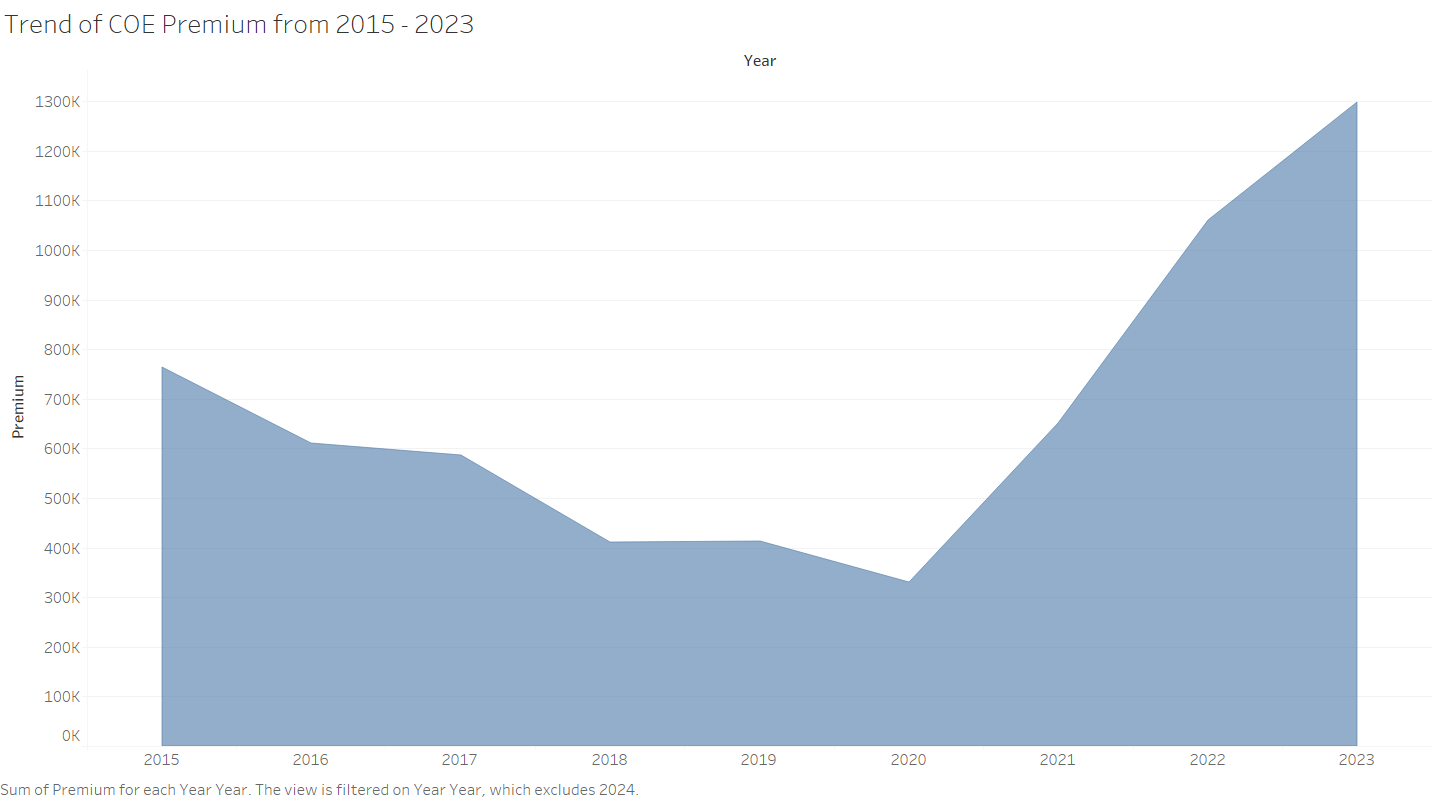
\includegraphics[width=.9\linewidth]{./charts/coe_premium.png}
\end{center}

\begin{itemize}
\item Visual encoding here includes:
\begin{itemize}
\item Position - Denoting the price of COE premium
\end{itemize}
\item Insights
\begin{itemize}
\item Steep increase in premium since 2019
\end{itemize}
\end{itemize}
\subsection{Correlation between COE quota, bids, and premium}
\label{sec:orgb0038a0}

\begin{center}
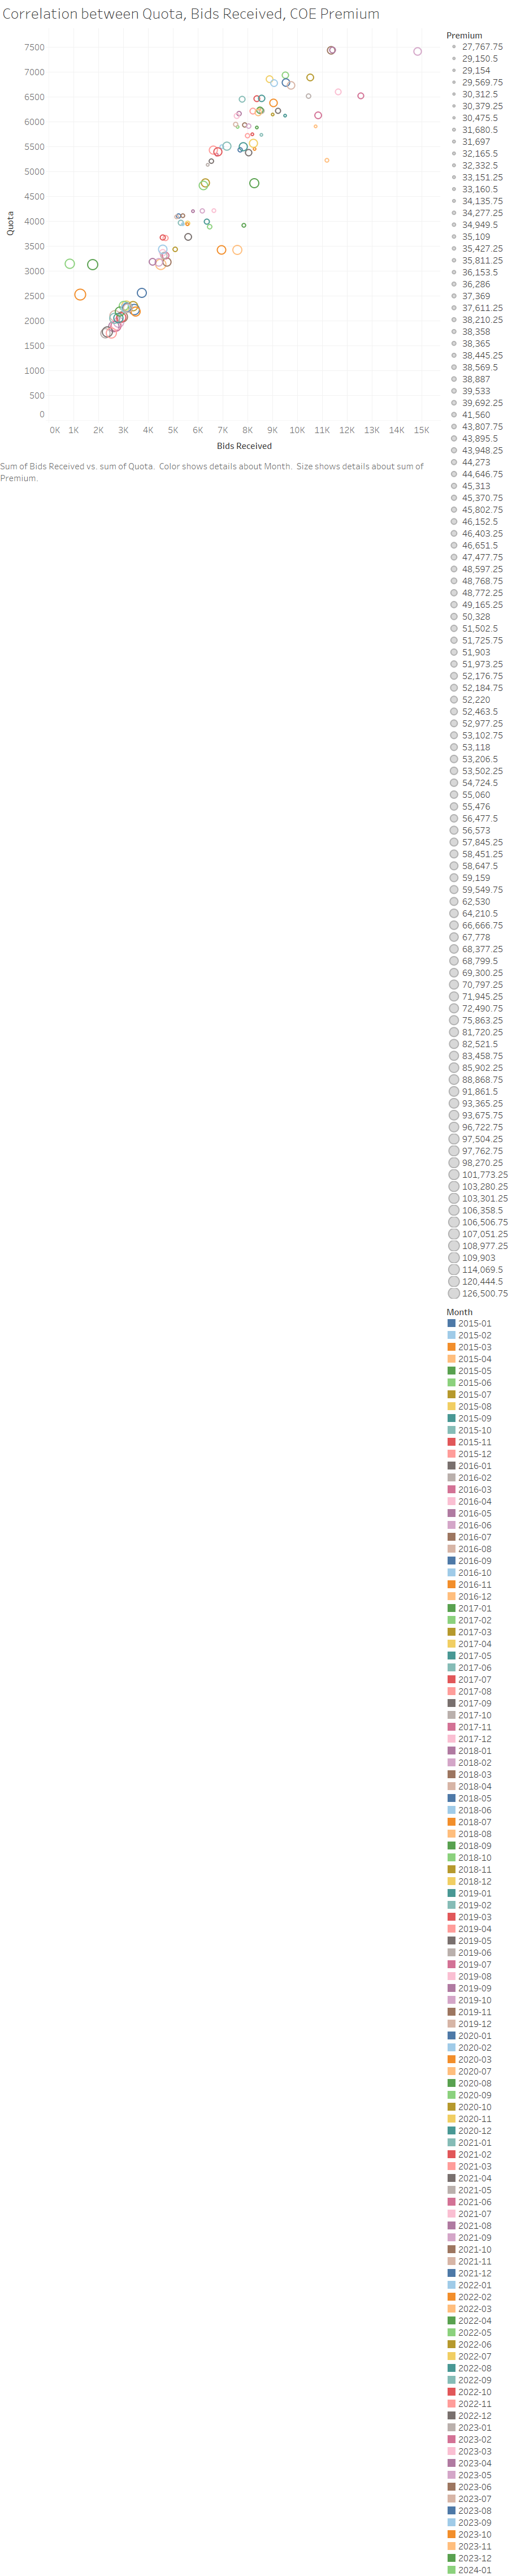
\includegraphics[width=.9\linewidth]{./charts/quota-bids-premium.png}
\end{center}

\begin{itemize}
\item A bubble chart was chosen to show the relationship between quota, bids and premium.
\item Visual encoding here includes:
\begin{itemize}
\item Position - Denoting both the number of COE quota and bids that month
\item Size - Denoting the amount of COE premium that month
\item Color - Differentiating the month (and making overlapping points clearer)
\end{itemize}
\item Insights
\begin{itemize}
\item Positive correlation between COE quota and bids
\item Additionally, not enough evidence to suggest that high COE premiums leads to lower bids and quota but there seems to be such a trend.
\end{itemize}
\end{itemize}
\subsection{Correlation between revalidation, bids, and premium}
\label{sec:orgea7255f}

\begin{center}
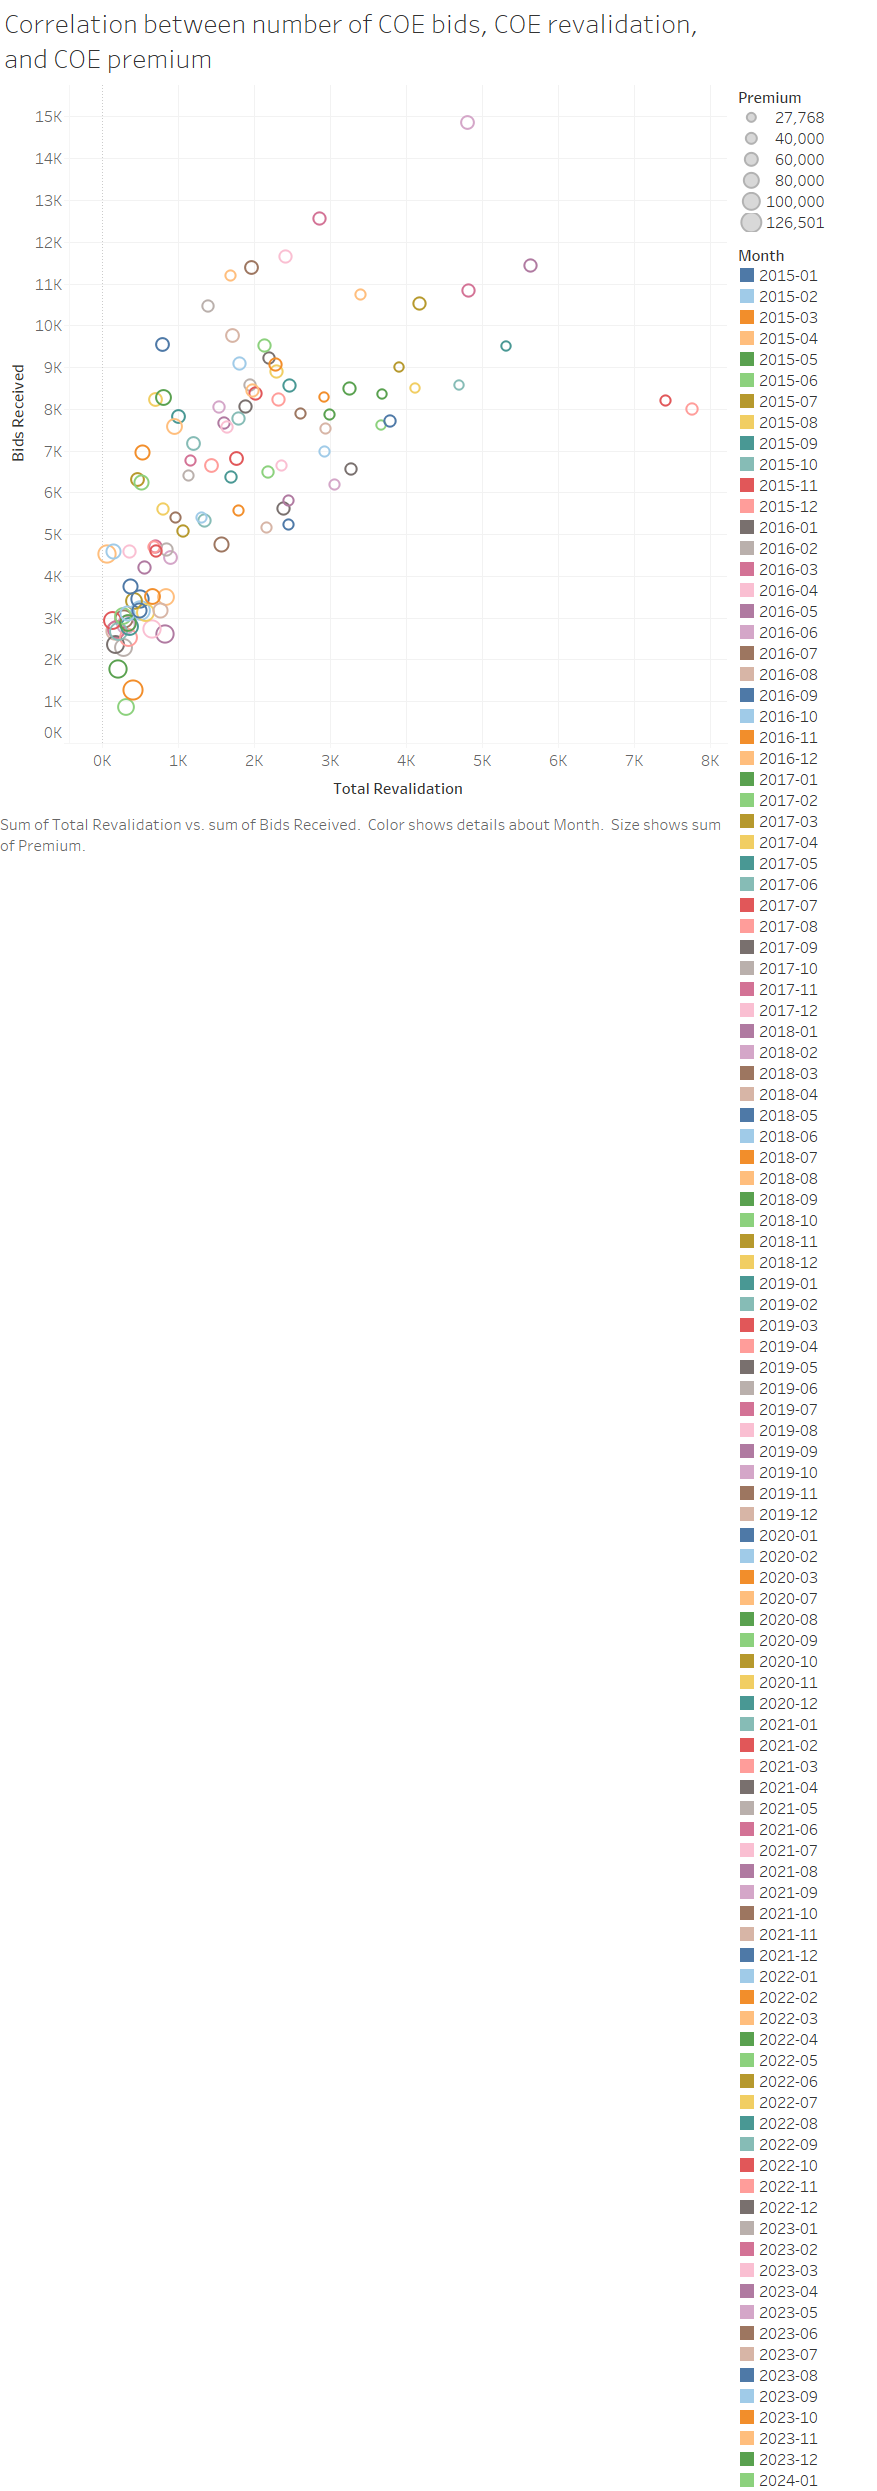
\includegraphics[width=.9\linewidth]{./charts/reval-bids-premium.png}
\end{center}

\begin{itemize}
\item An bubble chart was chosen to emphasise the correlation between the three variables.
\item Visual encoding here includes:
\begin{itemize}
\item Position - Denoting the number of COE revalidations and bids that month
\item Size - Denoting the amount of COE premium that month
\item Color - Differentiating the month (and making overlapping points clearer)
\end{itemize}
\item Insights
\begin{itemize}
\item Clear correlation between the three variables
\item High COE premiums lead to both lower revalidation and bids
\item And revalidation and bids positively correlated to each other
\end{itemize}
\end{itemize}
\end{document}
